\documentclass[aspectratio=169, table, 12pt]{beamer}

\usepackage{colortbl}
\usepackage{xcolor}
\usepackage{listings}
\usepackage{tabularx}
\usepackage{tikz}
\usetikzlibrary{arrows.meta, positioning, calc, fit,
  shapes.geometric, backgrounds}

\makeatletter
\def\input@path{{../theme/}}
\makeatother
\graphicspath{{../theme/}{../../figures/}}
\usetheme{Pradita}

\definecolor{praditagreen}{RGB}{37, 113, 71}

% Tema membuat garis tabel berwarna putih. Dikembalikan agar tabel terbaca.
\arrayrulecolor{black}
\setlength{\arrayrulewidth}{0.5pt}

% Menempatkan gambar di tengah kolom, mendatar sekaligus tegak. Lebarnya
% dipenuhi selebar kolom. Bila hasilnya melebihi tinggi yang disediakan,
% tingginya yang menjadi pembatas, sehingga gambar tidak menembus bingkai.
\newsavebox{\kotakkolom}
\newcommand{\gambarkolom}[2][0.72\textheight]{%
  \sbox{\kotakkolom}{\resizebox{\linewidth}{!}{#2}}%
  \begin{minipage}[c][#1][c]{\linewidth}%
    \centering
    \ifdim\dimexpr\ht\kotakkolom+\dp\kotakkolom\relax>#1\relax
      \resizebox{!}{#1}{#2}%
    \else
      \usebox{\kotakkolom}%
    \fi
  \end{minipage}%
}

\lstdefinestyle{PythonStyle}{
  language=Python,
  basicstyle=\ttfamily\scriptsize,
  keywordstyle=\color{blue}\bfseries,
  commentstyle=\color{gray}\itshape,
  stringstyle=\color{red},
  breaklines=true,
  frame=lines,
  backgroundcolor=\color{lightgray!10},
  tabsize=2,
  showstringspaces=false
}

\lstdefinelanguage{bash}{
  keywords={},
  basicstyle=\ttfamily\scriptsize,
  ndkeywords={cd, python, bash, source},
  ndkeywordstyle=\color{purple}\bfseries,
  sensitive=true,
  commentstyle=\color{gray},
  breaklines=true,
  frame=lines,
  backgroundcolor=\color{lightgray!10},
  tabsize=2,
  comment=[l]{\#},
  showstringspaces=false
}

\title{\Huge{Space-Based Architecture}}
\subtitle{IF231303 Arsitektur Perangkat Lunak}
\author{Alfa Yohannis}

\begin{document}

\frame{\titlepage}

\begin{frame}{{\Large Tujuan Pembelajaran}}
  \vspace{10pt}
  \begin{enumerate}
    \item Menjelaskan bagian susunan berbasis \textit{tuple space} beserta peran
          ruang yang menggantikan basis data di jalur permintaan.
    \item Membedakan jalur data yang melewati basis data dari jalur data yang
          melewati memori, lalu menentukan kapan masing-masing layak dipilih.
    \item Mengukur \textit{throughput scaling}, \textit{stale read}, dan
          \textit{data loss} pada kedua versi.
  \end{enumerate}

  \vspace{10pt}
  {\small Contohnya pemroses setoran valuta asing, dibuat dua versi dengan
  domain yang sama persis.}
\end{frame}

\begin{frame}{{\Large Pendahuluan}}
  \vspace{8pt}
  \begin{itemize}\small
    \item Aplikasi dapat disalin ke sepuluh mesin tanpa kesulitan berarti.
          Basis datanya tidak.
    \item Ketika kesepuluh salinan menulis ke satu \textit{file} yang sama,
          giliran menulis itulah yang menentukan hasil akhirnya.
    \item Jalan keluarnya membalik kebiasaan, yaitu data yang dibutuhkan setiap
          permintaan dipindahkan ke memori tiap unit.
    \item Penyimpanan ke basis data dikerjakan belakangan, di luar jalur
          permintaan.
  \end{itemize}

  \vspace{8pt}
  {\small Gagasan ruang bersamanya sendiri sudah berumur empat dekade, yaitu
  bahasa Linda yang diperkenalkan Gelernter pada 1985.}
\end{frame}

\begin{frame}{{\Large Istilah yang Dipakai}}
  \vspace{10pt}
  \begin{itemize}\small
    \item \textbf{Tugas} adalah satu \textit{file} setoran berisi tiga ribu
          transaksi yang dikonversi lalu dijumlahkan.
    \item \textbf{\textit{Processing unit}} adalah proses yang mengerjakan tugas
          memakai data di memorinya sendiri.
    \item \textbf{Ruang} adalah tempat bersama untuk menaruh dan mengambil
          tupel, yaitu \textit{tuple space}.
    \item \textbf{Grid} adalah salinan data di dalam memori satu unit, dan
          isinya disegarkan berkala dari ruang.
  \end{itemize}

  \vspace{10pt}
  {\small Yang diukur bab ini tiga, yaitu tugas per detik, pembacaan yang
  memakai kurs kedaluwarsa, dan tugas yang lenyap ketika satu unit mati.}
\end{frame}

\begin{frame}{{\Large Bagian Susunannya}}
  \vspace{10pt}
  \centering
  \resizebox{0.80\textwidth}{!}{%
  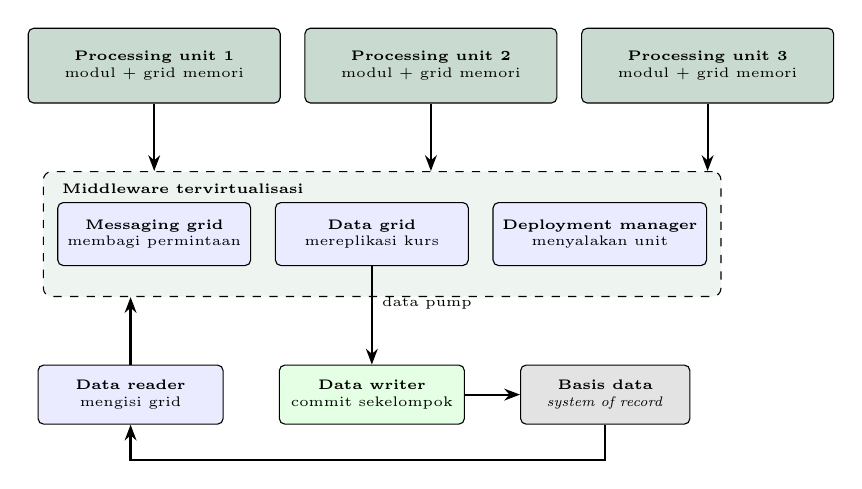
\begin{tikzpicture}[
      kotak/.style={draw, rounded corners=2pt, align=center,
        font=\tiny\bfseries},
      unit/.style={kotak, fill=praditagreen!25, minimum width=3.2cm,
        minimum height=0.95cm},
      bagian/.style={kotak, fill=blue!8, minimum width=2.45cm,
        minimum height=0.8cm},
      simpan/.style={kotak, fill=green!10, minimum width=2.35cm,
        minimum height=0.75cm},
      panah/.style={-{Stealth[length=2mm]}, thick}
    ]
      \node[unit] (u1) {Processing unit 1\\
        {\tiny\mdseries modul + grid memori}};
      \node[unit, right=0.3cm of u1] (u2) {Processing unit 2\\
        {\tiny\mdseries modul + grid memori}};
      \node[unit, right=0.3cm of u2] (u3) {Processing unit 3\\
        {\tiny\mdseries modul + grid memori}};
  
      \node[bagian, below=1.25cm of u1] (pesan) {Messaging grid\\
        {\tiny\mdseries membagi permintaan}};
      \node[bagian, right=0.3cm of pesan] (data) {Data grid\\
        {\tiny\mdseries mereplikasi kurs}};
      \node[bagian, right=0.3cm of data] (kelola) {Deployment manager\\
        {\tiny\mdseries menyalakan unit}};
  
      \begin{scope}[on background layer]
        \node[draw, dashed, rounded corners=3pt, fill=praditagreen!8,
          inner ysep=11pt, inner xsep=5pt, fit=(pesan)(data)(kelola)] (mw) {};
      \end{scope}
      \node[font=\tiny\bfseries, anchor=north west]
        at ([shift={(0.12cm,-0.04cm)}]mw.north west) {Middleware tervirtualisasi};
  
      \node[simpan, below=1.25cm of data] (penulis) {Data writer\\
        {\tiny\mdseries commit sekelompok}};
      \node[simpan, left=0.7cm of penulis, fill=blue!8] (pembaca) {Data reader\\
        {\tiny\mdseries mengisi grid}};
      \node[kotak, fill=gray!22, right=0.7cm of penulis, minimum width=2.15cm,
        minimum height=0.75cm] (basis) {Basis data\\
        {\tiny\mdseries \textit{system of record}}};
  
      \draw[panah] (u1) -- (u1|-mw.north);
      \draw[panah] (u2) -- (u2|-mw.north);
      \draw[panah] (u3) -- (u3|-mw.north);
      \draw[panah] (data) -- node[right, font=\tiny\mdseries, pos=0.38]
        {data pump} (penulis);
      \draw[panah] (penulis) -- (basis);
      \draw[panah] (basis) |- ([yshift=-0.45cm]pembaca.south) -- (pembaca);
      \draw[panah] (pembaca) -- (pembaca|-mw.south);
    \end{tikzpicture}}

  \vspace{10pt}
  \raggedright
  {\small Tidak ada panah dari \textit{processing unit} yang langsung menuju
  basis data.}
\end{frame}

\begin{frame}{{\Large Wujudnya pada Kode Bab Ini}}
  \vspace{8pt}
  \centering
  \small
  \begin{tabularx}{0.96\textwidth}{|l|X|l|}
    \hline
    \textbf{Bagian} & \textbf{Tugasnya} & \textbf{Pada bab ini} \\
    \hline
    \textit{Processing unit} & Mengerjakan permintaan memakai data di memorinya sendiri & \texttt{UnitRuang} \\
    \hline
    \textit{Messaging grid} & Membagikan permintaan kepada unit yang menganggur & \texttt{Ruang} \\
    \hline
    \textit{Data grid} & Menyimpan data bersama lalu mereplikasinya & \texttt{Ruang} \\
    \hline
    \textit{Data pump} & Memindahkan hasil ke basis data di luar jalur permintaan & \texttt{PenulisData} \\
    \hline
    \textit{Deployment manager} & Menyalakan unit mengikuti beban & tidak dibuat \\
    \hline
  \end{tabularx}
\end{frame}

\begin{frame}{{\Large \textit{Tuple Space} dan Tiga Operasinya}}
  \vspace{8pt}
  \centering
  \small
  \begin{tabularx}{0.96\textwidth}{|l|l|X|}
    \hline
    \textbf{Linda} & \textbf{Kelas \texttt{Ruang}} & \textbf{Akibatnya pada isi ruang} \\
    \hline
    \texttt{out} & \texttt{tulis} & Tupel bertambah satu, penulisnya tidak menunggu siapa pun \\
    \hline
    \texttt{in} & \texttt{ambil} & Tupel yang cocok dikeluarkan, hanya satu pengambil yang mendapatkannya \\
    \hline
    \texttt{rd} & \texttt{baca} & Tupel yang cocok disalin, dan tetap tinggal bagi pembaca lain \\
    \hline
  \end{tabularx}

  \vspace{8pt}
  \raggedright
  {\small Tugas ditulis lalu diambil, sehingga satu tugas dikerjakan tepat satu
  unit. Kurs ditulis lalu dibaca, sehingga seluruh unit memperoleh kurs yang
  sama tanpa saling menunggu.}
\end{frame}

\begin{frame}{{\Large Analogi: Papan Pengumuman}}
  \vspace{10pt}
  \begin{itemize}\small
    \item Petugas menempel selembar pengumuman lalu pergi, tanpa tahu siapa yang
          akan membacanya.
    \item Pengumuman itu tetap menempel walaupun petugasnya sudah pulang, dan
          dibaca banyak orang.
    \item Di sebelahnya tergantung setumpuk formulir cuti. Formulir yang sudah
          diambil satu mahasiswa tidak mungkin diambil mahasiswa berikutnya.
  \end{itemize}

  \vspace{10pt}
  {\small Pengumuman itulah \texttt{baca}, formulir itulah \texttt{ambil}, dan
  papannya itulah ruang.}
\end{frame}

\begin{frame}[fragile]{{\Large Kode: \texttt{ambil} dan \texttt{baca}}}
  \vspace{4pt}
\begin{lstlisting}[style=PythonStyle]
def ambil(self, pola: tuple, batas_waktu: float | None = None):
  # Mengeluarkan satu tupel yang memenuhi pola dari ruang.
  return self._tunggu_cocok(pola, True, batas_waktu)

def baca(self, pola: tuple, batas_waktu: float | None = None):
  # Membaca satu tupel yang memenuhi pola tanpa mengeluarkannya.
  return self._tunggu_cocok(pola, False, batas_waktu)
\end{lstlisting}

  \vspace{4pt}
  {\small Keduanya memanggil penolong yang sama, dan yang membedakannya hanya
  satu argumen. Pencarian dan pengeluaran dikerjakan di bawah satu kunci yang
  sama, sehingga dua pengambil atas satu tupel selalu menghasilkan satu
  pemenang.}
\end{frame}

\begin{frame}{{\Large \textit{Class Diagram}: Dua Jalur Data}}
  \vspace{4pt}
  \begin{center}
    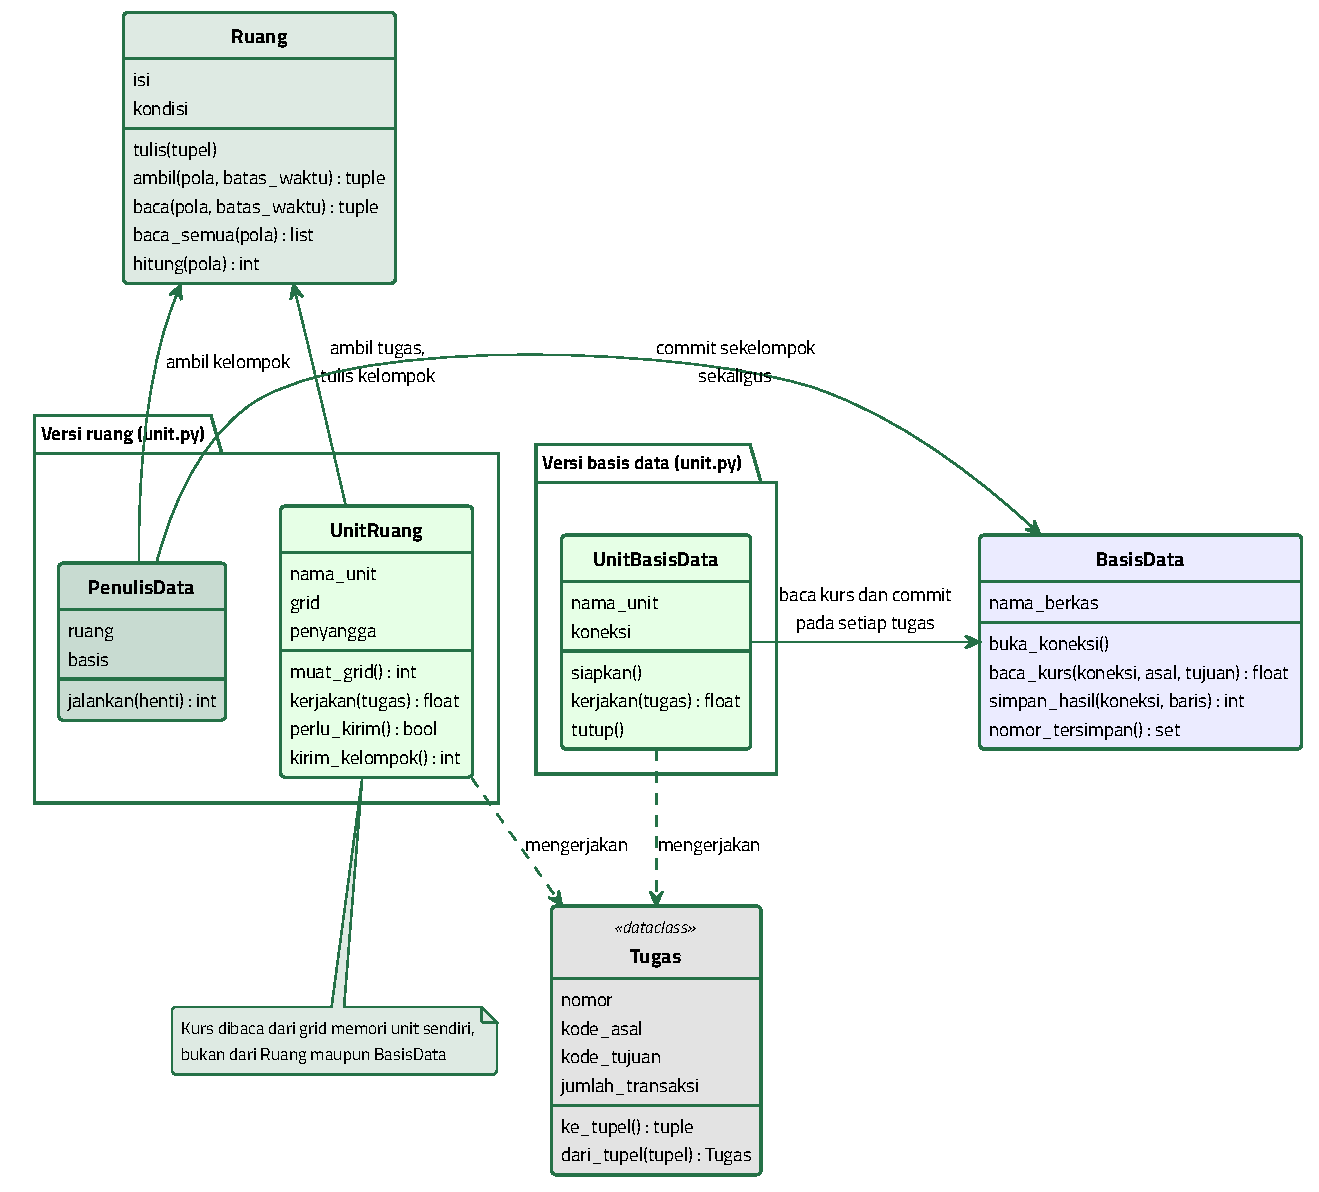
\includegraphics[width=\textwidth, height=0.74\textheight,
      keepaspectratio]{kelas-ruang.pdf}
  \end{center}
\end{frame}

\begin{frame}{{\Large Penjelasan \textit{Class Diagram}}}
  \vspace{10pt}
  \begin{itemize}\small
    \item \texttt{UnitBasisData} menunjuk langsung ke \textit{file} SQLite,
          sehingga basis datanya berada di jalur setiap tugas.
    \item \texttt{UnitRuang} hanya menunjuk ke ruang, dan tidak mengenal
          \textit{file} sama sekali.
    \item \texttt{PenulisData} yang menyambungkan ruang dengan \textit{file},
          dan jalannya di luar jalur permintaan.
    \item Domainnya sama persis pada kedua versi, yaitu \texttt{Tugas} beserta
          fungsi hitungnya.
  \end{itemize}

  \vspace{10pt}
  {\small Yang layak diperhatikan arah panahnya, bukan jumlah kelasnya.}
\end{frame}

\begin{frame}[fragile]{{\Large Kode: Versi Basis Data}}
  \vspace{4pt}
\begin{lstlisting}[style=PythonStyle]
def kerjakan(self, tugas: domain.Tugas) -> float:
  # Membaca kurs, menghitung total, lalu menyimpannya dalam satu commit.
  mulai = time.perf_counter()
  kurs = self.basis.baca_kurs(self.koneksi, tugas.kode_asal,
                              tugas.kode_tujuan)
  total = domain.hitung_total(tugas, kurs)
  self.basis.simpan_hasil(self.koneksi,
                          [(tugas.nomor, self.nama_unit, total)])
  return (time.perf_counter() - mulai) * 1000.0
\end{lstlisting}

  \vspace{4pt}
  {\small Ketiga langkahnya, yaitu membaca kurs, menghitung, dan menyimpan,
  seluruhnya berada di jalur setiap tugas.}
\end{frame}

\begin{frame}[fragile]{{\Large Kode: Versi Ruang}}
  \vspace{4pt}
\begin{lstlisting}[style=PythonStyle]
def kerjakan(self, tugas: domain.Tugas) -> float:
  # Menghitung total tugas memakai kurs lokal, lalu menumpuk hasilnya.
  mulai = time.perf_counter()
  kurs = self.grid.get((tugas.kode_asal, tugas.kode_tujuan))
  total = domain.hitung_total(tugas, kurs)
  self.penyangga.append((tugas.nomor, self.nama_unit, total))
  if self.perlu_kirim():
    self.kirim_kelompok()
  return (time.perf_counter() - mulai) * 1000.0
\end{lstlisting}

  \vspace{4pt}
  {\small Penyangga dikirim bila sudah berisi lima puluh hasil atau sudah
  tertahan lebih dari 0,25 detik. Apache Ignite menyebut cara itu
  \textit{write-behind}.}
\end{frame}

\begin{frame}{{\Large \textit{Sequence Diagram}: Satu Tugas}}
  \vspace{4pt}
  \begin{center}
    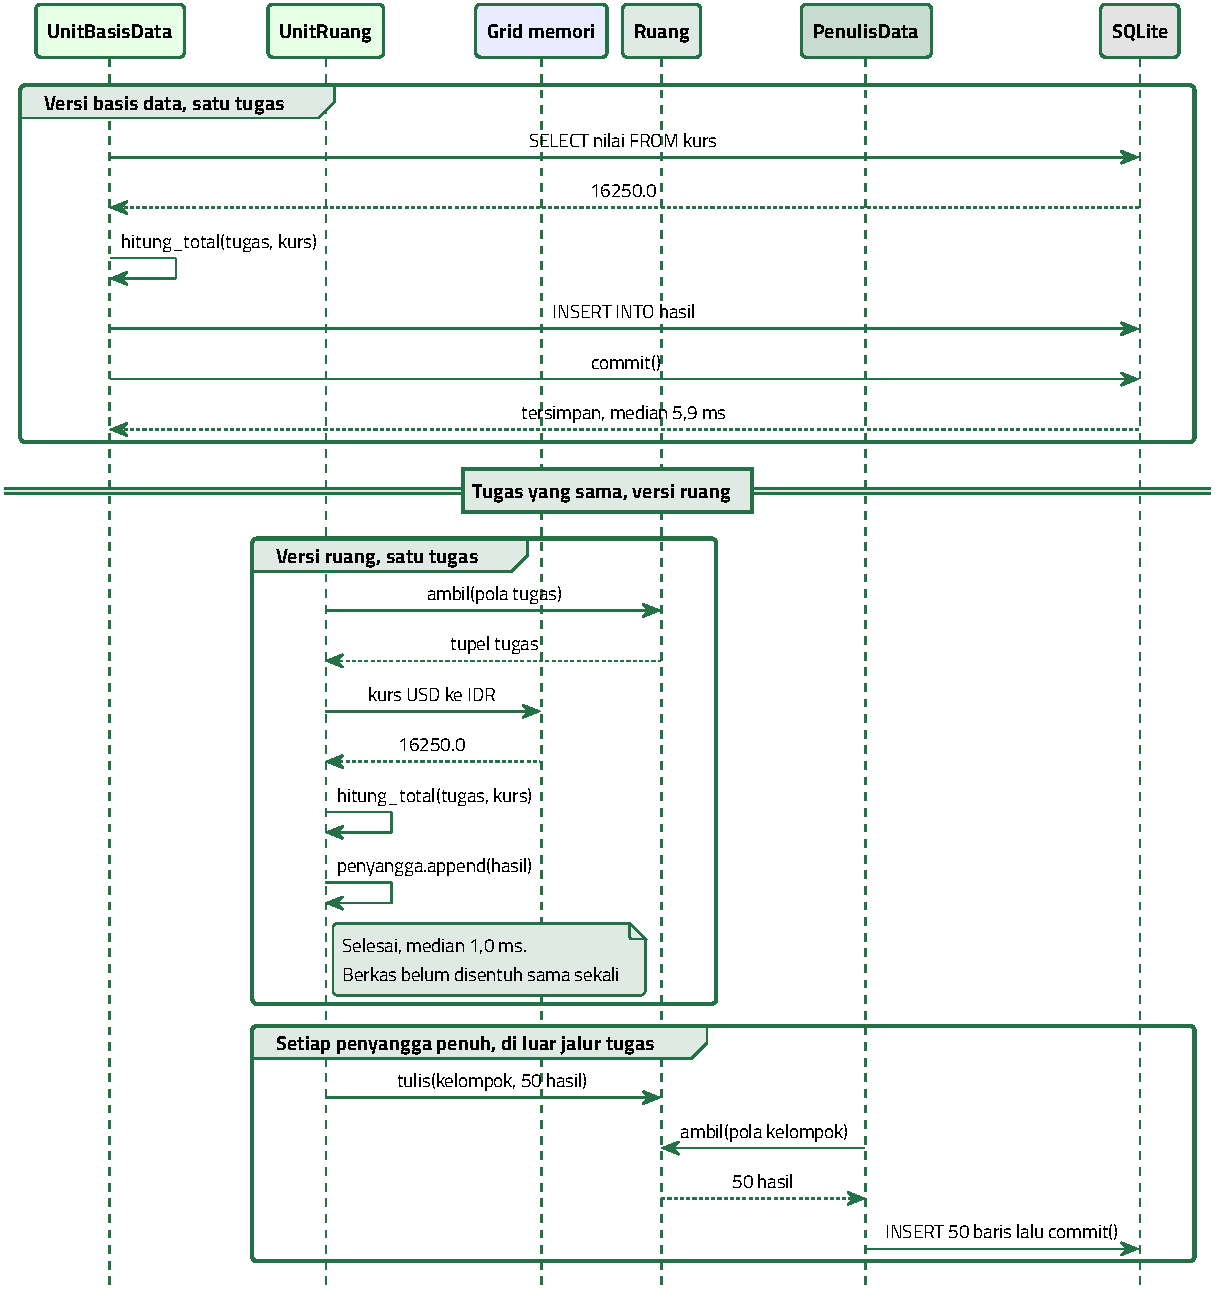
\includegraphics[width=\textwidth, height=0.74\textheight,
      keepaspectratio]{sekuens-ruang.pdf}
  \end{center}
\end{frame}

\begin{frame}{{\Large Penjelasan \textit{Sequence Diagram}}}
  \vspace{10pt}
  \begin{itemize}\small
    \item Perhitungannya sama persis pada kedua versi, yang berbeda apa yang
          ditunggu sesudahnya.
    \item Versi basis data menunggu \textit{commit} selesai sebelum tugasnya
          dinyatakan selesai.
    \item Versi ruang selesai begitu hasilnya masuk penyangga, dan pengiriman ke
          ruang menyusul belakangan.
    \item Akibatnya berlawanan arah, yaitu lebih cepat, tetapi hasilnya belum
          tersimpan di mana pun kecuali memori satu unit.
  \end{itemize}
\end{frame}

\begin{frame}{{\Large Hasil: \textit{Throughput Scaling}}}
  \vspace{6pt}
  {\small Beban tetap 900 tugas, lima putaran tiap susunan, berselang-seling.}

  \vspace{6pt}
  \centering
  \small
  \begin{tabularx}{0.96\textwidth}{|l|X|X|l|}
    \hline
    \textbf{Unit} & \textbf{Basis data, tugas/detik} & \textbf{Ruang, tugas/detik} & \textbf{Perbandingan} \\
    \hline
    1 & 319,1 & 1307,7 & 4,1 kali \\
    \hline
    2 & 298,6 & 2457,1 & 8,2 kali \\
    \hline
    4 & 244,3 & 3594,1 & 14,7 kali \\
    \hline
    8 & 273,0 & 4007,5 & 14,7 kali \\
    \hline
  \end{tabularx}
\end{frame}

\begin{frame}{{\Large Membaca Hasilnya}}
  \vspace{10pt}
  \begin{itemize}\small
    \item Versi basis data tidak bertambah hasilnya, bahkan turun dari 319,1
          menjadi 244,3 tugas per detik. Menambah unit hanya menambah pengantre
          pada \textit{file} yang sama.
    \item Versi ruang naik, tetapi tidak sebanding jumlah unitnya, yaitu 2,7
          kali pada empat unit. Laptop percobaannya berinti empat.
    \item Median latensi versi basis data hanya naik dari 3,118 ms menjadi 4,250
          ms, sedangkan nilai terbesarnya melonjak menjadi 1936,111 ms.
  \end{itemize}

  \vspace{10pt}
  {\small Lonjakan pada nilai terbesar itulah tanda antrean, dan median
  menyembunyikannya.}
\end{frame}

\begin{frame}{{\Large Hasil: \textit{Stale Read}}}
  \vspace{6pt}
  {\small Kurs terbit tiap 50 ms, empat pembaca, tiga putaran satu detik tiap
  jeda.}

  \vspace{6pt}
  \centering
  \small
  \begin{tabularx}{0.9\textwidth}{|r|r|r|X|}
    \hline
    \textbf{\textit{Replication lag}} & \textbf{Pembacaan} & \textbf{Basi} & \textbf{Bagian basi} \\
    \hline
    0 ms & 11.048 & 0 & 0,0\% \\
    \hline
    10 ms & 11.029 & 1.034 & 9,4\% \\
    \hline
    25 ms & 11.046 & 2.519 & 22,8\% \\
    \hline
    50 ms & 11.067 & 1.052 & 9,5\% \\
    \hline
    200 ms & 11.056 & 8.564 & 77,5\% \\
    \hline
  \end{tabularx}

  \vspace{6pt}
  \raggedright
  {\small Baris 50 ms menyimpang sebab jedanya sama persis dengan jarak terbit
  kurs, sehingga penyegaran selalu tiba sesaat sesudah kurs baru terbit.}
\end{frame}

\begin{frame}{{\Large Kasus: Pengisian Rencana Studi}}
  \vspace{8pt}
  \begin{enumerate}\small
    \item Sisa kuota setiap kelas disalin ke grid memori tiap unit, dengan
          replikasi setiap dua ratus milidetik.
    \item Pada menit pertama pembukaan, ribuan mahasiswa menekan tombol yang
          sama.
    \item Belasan unit membaca sisa kuota yang sama dari grid masing-masing,
          lalu sama-sama menyimpulkan kursinya masih ada.
    \item Kelas berkuota empat puluh terisi lima puluh tiga mahasiswa.
  \end{enumerate}

  \vspace{8pt}
  {\small Tiga belas mahasiswa terpaksa dikeluarkan keesokan harinya. Pada jeda
  200 ms, 77,5 persen pembacaan memang basi.}
\end{frame}

\begin{frame}{{\Large Hasil: \textit{Data Loss}}}
  \vspace{6pt}
  {\small Empat unit mengerjakan 600 tugas, satu unit dimatikan dengan SIGKILL
  pada separuh beban.}

  \vspace{6pt}
  \centering
  \small
  \begin{tabularx}{0.9\textwidth}{|X|l|l|}
    \hline
    \textbf{Yang dilaporkan} & \textbf{Basis data} & \textbf{Ruang} \\
    \hline
    Median tugas hilang & 1 & 28 \\
    \hline
    \textit{Range} tugas hilang & 1 sampai 1 & 15 sampai 41 \\
    \hline
    Transaksi hilang pada median & 3.000 & 84.000 \\
    \hline
  \end{tabularx}

  \vspace{6pt}
  \raggedright
  {\small Yang hilang adalah isi penyangga unit itu, dan jumlahnya bergantung
  pada seberapa penuh penyangganya saat unitnya mati.}
\end{frame}

\begin{frame}{{\Large Ukuran Kelompok sebagai Tombol}}
  \vspace{10pt}
  \begin{itemize}\small
    \item Besar kehilangan bukan sifat bawaan susunannya, melainkan akibat satu
          angka yang dapat diubah.
    \item Dengan ukuran kelompok satu, kehilangannya turun menjadi satu tugas,
          sama dengan versi basis data.
    \item Hasil per detiknya pada empat unit tercatat 3366,2, sedangkan dengan
          ukuran kelompok lima puluh tercatat 3594,1.
  \end{itemize}

  \vspace{10pt}
  {\small Harga keamanan itu sekitar enam persen hasil pada mesin percobaan ini,
  dan Latihan 3 meminta angkanya diukur ulang di mesin sendiri.}
\end{frame}

\begin{frame}{{\Large \textit{Summary}}}
  \vspace{10pt}
  \begin{itemize}\small
    \item Ruang menggantikan basis data di jalur permintaan, dan basis datanya
          dijangkau lewat \textit{data pump} di belakang.
    \item Pengambilan mengeluarkan tupel sehingga satu tugas dikerjakan tepat
          satu unit, sedangkan pembacaan menyalinnya.
    \item Versi basis data tidak bertambah hasilnya ketika unitnya ditambah,
          sedangkan versi ruang naik sampai 14,7 kali.
    \item Kecepatan itu ditebus dua kali, yaitu kurs basi dan hasil yang lenyap
          bersama unit yang mati.
  \end{itemize}

  \vspace{10pt}
  {\small Pesan utamanya, memindahkan penyimpanan ke luar jalur permintaan
  membeli hasil per detik dengan membayar ketepatan data pada saat yang paling
  buruk.}
\end{frame}

\begin{frame}[fragile]{{\Large Persiapan Latihan}}
  \vspace{5pt}
\begin{lstlisting}[language=bash]
bash sources/siapkan_venv.sh
source .venv/bin/activate
cd sources/chapter08
python unit.py ruang 4
# Tugas per detik : 3815.9
# Tugas tersimpan : 900
\end{lstlisting}

  \vspace{6pt}
  {\small Bab ini hanya memakai pustaka standar Python. Langkah lengkap, tabel
  contoh, dan lembar isian ada di modul Bab 8, yang menjadi rujukan utama
  latihan ini.}
\end{frame}

\begin{frame}[fragile]{{\Large Latihan 1: \textit{Throughput Scaling}}}
  \vspace{2pt}
  {\small Tujuan: menguji apakah menambah \textit{processing unit} benar-benar
  menambah hasil.}

  \vspace{2pt}
\begin{lstlisting}[language=bash]
python ukur_hasil.py
# 4 basis data  244.3 tugas/detik
# 4 ruang      3594.1 tugas/detik
\end{lstlisting}

  \vspace{2pt}
  \begin{enumerate}\small
    \item Catat tugas per detik, median, dan nilai terbesar untuk kedelapan
          baris.
    \item Hitung perbandingan kedua versi pada tiap jumlah unit.
    \item Ubah \texttt{JUMLAH\_UNIT} menjadi memuat 16, lalu catat apakah
          hasilnya masih naik.
  \end{enumerate}

  \vspace{2pt}
  {\small Pertanyaan: mengapa hasil versi basis data tidak naik?}
\end{frame}

\begin{frame}[fragile]{{\Large Latihan 2: \textit{Stale Read}}}
  \vspace{2pt}
  {\small Tujuan: mengukur ketepatan data yang ditebus demi kecepatan.}

  \vspace{2pt}
\begin{lstlisting}[language=bash]
python ukur_basi.py
#  25 ms  2519 basi  22.8%
# 200 ms  8564 basi  77.5%
\end{lstlisting}

  \vspace{2pt}
  \begin{enumerate}\small
    \item Catat ketiga kolom untuk ketujuh jeda.
    \item Jelaskan mengapa baris 50 ms lebih kecil daripada baris 25 ms.
    \item Ubah \texttt{JEDA\_PEMBARUAN} dari 0,05 menjadi 0,02 detik, lalu catat
          perubahannya.
  \end{enumerate}

  \vspace{2pt}
  {\small Pertanyaan: berapa jeda yang masih dapat diterima untuk pengisian
  rencana studi?}
\end{frame}

\begin{frame}[fragile]{{\Large Latihan 3: \textit{Data Loss}}}
  \vspace{2pt}
  {\small Tujuan: mengukur tebusan yang paling berat, yaitu hasil yang lenyap.}

  \vspace{2pt}
\begin{lstlisting}[language=bash]
python uji_kehilangan.py
# Median hilang, basis data : 1 tugas
# Median hilang, ruang      : 28 tugas
\end{lstlisting}

  \vspace{2pt}
  \begin{enumerate}\small
    \item Catat kedua kolom untuk kelima putaran beserta median dan
          \textit{range}-nya.
    \item Ubah \texttt{UKURAN\_KELOMPOK} dari 50 menjadi 1, lalu catat tugas
          yang hilang.
    \item Jalankan \texttt{python ukur\_hasil.py} dengan ukuran kelompok itu,
          lalu catat hasilnya pada empat unit.
  \end{enumerate}

  \vspace{2pt}
  {\small Pertanyaan: ukuran kelompok mana yang dipakai untuk penerimaan
  mahasiswa baru?}
\end{frame}

\end{document}
